\documentclass[aps, pre, onecolumn, nofootinbib, notitlepage, groupedaddress, amsfonts, amssymb, amsmath, longbibliography, superscriptaddress]{revtex4-1}
\usepackage{tabularx}
\usepackage{graphicx}
\usepackage{hyperref}
\usepackage{xcolor}
\usepackage{placeins}
\hypersetup{
    colorlinks,
    linkcolor={red!50!black},
    citecolor={blue!50!black},
    urlcolor={blue!80!black}
}
\usepackage{bm}
\usepackage{natbib}
\usepackage{longtable}
\LTcapwidth=0.87\textwidth

\newcommand{\Div}[1]{\ensuremath{\nabla\cdot\left( #1\right)}}
\newcommand{\DivU}{\ensuremath{\nabla\cdot\bm{u}}}
\newcommand{\angles}[1]{\ensuremath{\left\langle #1 \right\rangle}}
\newcommand{\KS}[1]{\ensuremath{D_{\text{KS}}(#1)}}
\newcommand{\KSstat}[1]{\ensuremath{\overline{D_\text{KS}(#1)}}}
\newcommand{\grad}{\ensuremath{\nabla}}
\newcommand{\RB}{Rayleigh-B\'{e}nard }
\newcommand{\Reff}{\ensuremath{\text{Re}_{\text{ff}}}}
\newcommand{\Peff}{\ensuremath{\text{Pe}_{\text{ff}}}}

\newcommand{\ea}[1]{{\color{red} #1}}

\newcommand\mnras{{MNRAS}}%
\newcommand\apjl{{The Astrophysical Journal Letters}}%

\begin{document}
\author{Evan H. Anders}
\affiliation{Dept. Astrophysical \& Planetary Sciences, University of Colorado -- Boulder, Boulder, CO 80309, USA}
\affiliation{Laboratory for Atmospheric and Space Physics, Boulder, CO 80303, USA}
\author{Geoffrey M. Vasil}
\affiliation{University of Sydney School of Mathematics and Statistics, Sydney, NSW 2006, Australia}
\author{Benjamin P. Brown}
\affiliation{Dept. Astrophysical \& Planetary Sciences, University of Colorado -- Boulder, Boulder, CO 80309, USA}
\affiliation{Laboratory for Atmospheric and Space Physics, Boulder, CO 80303, USA}
\author{Lydia Korre}
\affiliation{Laboratory for Atmospheric and Space Physics, Boulder, CO 80303, USA}

\title{Convective dynamics with mixed temperature boundary conditions: \\
why thermal relaxation matters and how to accelerate it}

\begin{abstract}
Astrophysical simulations of convection frequently impose different thermal boundary conditions at the top and the bottom of the domain in an effort to more accurately reflect the natural system being modeled.
In this work, we study \RB convection (RBC) with mixed (``FT'') temperature boundary conditions.
We aim to understand how FT boundaries change the nature of the convective solution compared to the traditional choice of fixing the temperature at the top and bottom of the domain (``TT'').
We find that simulations with FT boundaries experience a long thermal rundown while simulations with TT boundaries do not.
In the relaxed state, the mean behavior of an FT simulation corresponds to an equivalent simulation with TT boundaries.
The fast evolution of TT simulations can therefore be taken advantage of to rapidly relax FT simulations.
We show that these findings carry over to more complicated problems through a brief examination of rotating convection.
We furthermore find that FT boundaries introduce minor asymmetries into the flow fields, with the fixed flux boundary producing more extreme events than the fixed temperature boundary, but that these asymmetries do not appreciably affect the bulk flows.
We conclude that thermal relaxation occurs in two stages: (1) changes to the experimental energy reservoir and (2) changes to the stratification of the experiment.
Through the proper choice of boundary conditions or initial conditions, the first of these stages can be bypassed, and the second stage seems to be irrelevant for RBC.
\end{abstract}
\maketitle

%%%%%%%%%%%%
%%%%%%%%%%%
% INTRO
%%%%%%%%%%%
%%%%%%%%%%%%

\section{Introduction}
\label{sec:introduction}
Convection is a crucial heat transport mechanism in the atmospheres and interiors of stars and planets.
Numerical simulations are a commonly-used tool in studies of geophysical or astrophysical convection.
These studies range from examinations of convection in the simplified Boussinesq approximation \cite{spiegel&veronis1960, ahlers&all2009, plumley&julien2019} to highly complex ``dynamo simulations'' which include magnetism and atmospheric density stratification \cite{charbonneau2014, toomre2019}.
Regardless of complexity, numerically simulated convection is fundamentally driven by some combination of imposed boundary conditions and internal heating profiles \cite{goluskin2016}.
In studies of Boussinesq convection, the standard choice is to hold constant the temperature difference across the domain by fixing the temperature at the upper and lower boundaries.
However, a common choice of thermal boundary conditions in astrophysical convection \cite{glatzmaier&gilman1982, hurlburt&all1986, cattaneo&all1990, featherstone&hindman2016a, korre&all2019, wood&brummell2018, kapyla&all2019} is to fix the flux entering the domain through the bottom boundary and to fix the value of a thermodynamic quantity (e.g., temperature or entropy) at the top boundary.
%Mention mantle studies here
We are unaware of any study which has examined the consequences of imposing the ``mixed'' boundaries that are frequently favored in astrophysical convection studies.

In this work, we examine how the choice of using ``mixed'' boundaries affects the evolved nonlinear convective state in the simplest possible model: \RB convection (RBC) under the Boussinesq approximation.
In RBC, temperature is the only thermodynamic quantity and throughout this work we will \ea{adopt the gnomenclature of past authors including ref.~\cite{ishiwatari&all1994} and} refer to the choice of fixing the flux at the bottom and temperature at the top as ``FT'' boundary conditions.
We will refer to the common choice of fixing temperature at both boundaries as ``TT'' boundaries, and fixing the flux at both boundaries as ``FF'' boundaries\footnote{Note, in ref.~\cite{goluskin2016}, our TT, FF, and FT are respectively called RB1, RB2, and RB3.}.

\ea{Early studies of FF convection often focused on flow morphologies, as large-to-infinite aspect ratio convective rolls are linearly unstable at the critical value of the Rayleigh number (see e.g., ref.~\cite{chapman&proctor1980}).
However, the onset properties and resultant flow morphologies in FT simulations more strongly resemble TT dynamics than FF dynamics \cite{ishiwatari&all1994}.}
\ea{More recently,} FF and TT boundaries \ea{have been shown to} exhibit the same scaling of convective heat transport (quantified by the Nusselt number, Nu) as a function of increased convective driving (quantified by the Rayleigh number, Ra) \cite{johnston&doering2009}.
It is generally assumed that, \ea{in their statistically stationary states, simulations with} FT boundaries should behave similarly to FF boundaries \cite{goluskin2016, otero&all2002}.
%It is natural to assume that FT simulations should follow the same Nu vs.~Ra scaling laws as FF and TT boundary conditions.
However, FT boundaries introduce complexities into the convective solution which neither FF nor TT boundaries are exposed to.
First, the evolved mean temperature of a simulation with FT boundaries differs from the initial mean temperature, and therefore the thermal reservoir of the convective system must evolve (``relax'') over time \cite{anders&all2018}.
Second, FT boundary conditions are fundamentally asymmetric, and it is unclear if these asymmetries affect the evolved convective solution.

In this paper, we investigate the thermal relaxation of and the asymmetries in RBC with FT boundary conditions.
We also compare relaxed FT solutions to TT solutions.
\ea{When classical initial conditions which are in hydrostatic and thermal equilibrium are employed,} the thermal relaxation of FT systems is very long compared to TT systems, in which it is nearly instantaneous.
The thermal relaxation of FT simulations is analogous to a sweep through parameter space in which dynamics are sampled over a range of values of Ra.
We find that this long thermal relaxation can be bypassed by \ea{constructing smarter initial conditions based on the expected evolved Nusselt number, or by simply} using the results of TT simulations as initial conditions for FT simulations.
Finally, FT boundaries create some asymmetries in the convective flows, but these asymmetries do not meaningfully change the mean convective state compared to TT simulations.

We present these findings as follows.
In section \ref{sec:simulations}, we describe our simulation setup, numerical methods, \ea{initial conditions, and timescales in the convective systems}.
In section \ref{sec:results_timescales}, we describe our findings \ea{regarding} the time evolution of FT systems.
\ea{In section \ref{sec:results_dynamics}, we study dynamics and asymmetries in FT systems and compare them to TT systems.}
In section \ref{sec:results_rotating}, we show that these findings carry over to a more complex system (rotating \RB convection) with some interesting implications.
Finally, in section \ref{sec:discussion}, we summarize our findings and briefly describe the implications of this work for the field of astrophysical convection.

%%%%%%%%%%%%
%%%%%%%%%%%
% EXPERIMENT
%%%%%%%%%%%
%%%%%%%%%%%%
\section{Simulation Details}
\label{sec:simulations}
\ea{
\subsection{Equations, Control Parameters, Boundary Conditions, and Numerics}
}
We study incompressible RBC under a freefall nondimensionalization; for details of this nondimensionalization, we refer readers to our previous work \cite{anders&all2018}.
In section \ref{sec:results_rotating}, we study convection in the presence of vertical global rotation \cite{julien&all1996}, and include the Coriolis term in the momentum equation for generality.
The Boussinesq equations of motion are
\begin{align}
\DivU &= 0
	\label{eqn:incompressible}
\\
\frac{\partial \bm{u}}{\partial t} + \left(\bm{\omega} + \frac{1}{\text{Ek }\Reff}\hat{z}\right)\times\bm{u} 
&= - \grad \varpi + T_1\hat{z} - \frac{1}{\Reff}\grad\times\bm{\omega},
	\label{eqn:bouss_momentum}
\\
\frac{\partial T_1}{\partial t}  + \bm{u}\cdot\grad T_1 + w \frac{\partial T_0}{\partial z} 
&= \frac{1}{\Peff}\grad^2 T_1,
	\label{eqn:bouss_energy}
\end{align}
where $\bm{u} = (u, v, w)$ is the velocity, $T = T_0(z) + T_1(x, y, z, t)$ is the temperature (where $T_0$ is \ea{a background linearly unstable temperature profile} and $T_1$ are the fluctuations around that profile), $\varpi$ is the reduced kinematic pressure \cite{anders&all2018} which enforces the incompressibility constraint, and $\bm{\omega} = \grad \times \bm{u}$ is the vorticity.
The dimensionless control parameters are the Rayleigh (Ra), Prandtl (Pr), and Ekman (Ek) numbers, defined respectively as
\begin{equation}
\text{Ra} = \frac{g \alpha L_z^3 \Delta}{\nu\kappa} = \frac{(L_z\,u_{\text{ff}})^2}{\nu\kappa}, \qquad \text{Pr} = \frac{\nu}{\kappa}, \qquad \text{Ek} = \frac{\nu}{2\Omega L_z^2},
\end{equation}
where $u_{\text{ff}}$ is the freefall velocity, $g$ is the gravity, $\alpha$ is the coefficient of thermal expansion, $L_z$ is the domain depth, $\nu$ and $\kappa$ are respectively the viscous and thermal diffusivity, $\Omega$ is the global rotation frequency, and $\Delta$ is the nondimensional temperature scale (defined below).
These parameters set the freefall Reynolds (\Reff) and P\'{e}clet (\Peff) numbers, 
\begin{equation}
\Reff = \sqrt{\frac{\text{Ra}}{\text{Pr}}},\qquad
\Peff = \text{Pr }\Reff,
\end{equation}
and throughout this work we hold Pr = 1 so that $\Reff = \Peff$.
In non rotating RBC (section\ea{s} \ref{sec:results_timescales}\ea{\& \ref{sec:results_dynamics}}), we set Ek$\,= \infty$.

The extent of our numerical domain vertically is $z = [-0.5, 0.5]$ and horizontally is $x, y = [-\Gamma/2, \Gamma/2]$, where $\Gamma$ is the aspect ratio.
The \ea{background} temperature profile, $T_0(z) = 0.5 - z$, is unstable and linearly decreases from a value of 1 to 0 across the domain. 
The temperature scale, $\Delta$, is set by \ea{either} the temperature jump across the domain ($\Delta = \Delta T_0 =  T_0(z=0.5)-T_0(z=-0.5)$) for TT boundaries or by the temperature gradient length scale ($\Delta = L_z \partial_z T_0$) for FT boundaries.
We respectively define a temperature (Ra$_{\Delta T}$) and a flux (Ra$_{\partial_z T}$) Rayleigh number for these cases,
\begin{equation}
\text{Ra}_{\Delta T} = \frac{g \alpha L_z^3 \Delta T_0}{\nu\kappa}, \qquad 
\text{Ra}_{\partial_z T} = \frac{g \alpha L_z^4 \partial_z T_0}{\nu\kappa}.
\end{equation}
We impose FT and TT boundary conditions respectively as
\begin{equation}
(\text{FT}): \partial_z T_1 = 0 \text{ at $z$ = -0.5} \,\,\,\&\,\,\, T_1 = 0 \text{ at $z$ = 0.5};\qquad\qquad
(\text{TT}): T_1 = 0 \text{ at $z$ = \{-0.5, 0.5\}}.
\end{equation}

In section\ea{s} \ref{sec:results_timescales}\ea{\& \ref{sec:results_dynamics}}, we study \ea{non rotating convection}.
For comparison with the literature, we specify $\Gamma = 2$ and these simulations employ no-slip, impenetrable boundaries,
\begin{equation}
u = \ea{v =} w = 0 \, \, \text{at}\,\,z = \{-0.5, 0.5\}.
\label{eqn:vel_bcs}
\end{equation}
For this choice of \ea{aspect ratio and} boundary conditions, the critical value of the Rayleigh number is Ra$_{\partial_z T} = 1296$ for FT boundaries and Ra$_{\Delta T} = 1708$ for TT boundaries \cite{goluskin2016}.
Due to this difference in onset, it is reasonable to expect important differences between FT and TT solutions at low supercriticalities.
However, for the supercriticalities of O($10^{5+}$) studied in Sec.~\ref{sec:results_timescales}, we do not expect this difference in linear stability to be very important.
\ea{Many of these simulations are restricted to} two-dimensional (2D) convection \ea{by setting} $\partial_y = v = 0$.

The rotating cases in section \ref{sec:results_rotating} employ stress-free, impenetrable boundaries,
\begin{equation}
\partial_z u = \partial_z v = w = 0 \, \, \text{at}\,\,z = \{-0.5, 0.5\}.
\label{eqn:vel_bcs}
\end{equation}
We follow previous work  \cite{stellmach&all2014} and study three-dimensional (3D) tall, skinny boxes with $\Gamma = 10\lambda_c(\text{Ek})$, where $\lambda_c(\text{Ek})$ is the wavelength of convective onset at the specified value of Ek. 
For the cases studied here at Ek = $10^{-6}$, and for TT boundaries, $\lambda_c(10^{-6}) \approx 4.81 \times 10^{-2}$ and the critical Rayleigh number is Ra$_{\Delta T} \approx 9.2 \times 10^{8}$.

We utilize the Dedalus\footnote{\url{http://dedalus-project.org/}} pseudospectral framework \cite{burns&all2016, burns&all2019} to evolve Eqs.~(\ref{eqn:incompressible}-\ref{eqn:bouss_energy}) forward in time.
Our 2D simulations use an implicit-explicit (IMEX), third-order, four-stage Runge-Kutta timestepping scheme RK443; our 3D simulations use the \ea{IMEX}, second-order, two-stage Runge-Kutta scheme RK222 \cite{ascher&all1997}. 
The code used to run simulations and to create the figures in this work are available publicly online in a repository of supplemental materials \cite{anders&all2020a_supp}\footnote{Simulations were conducted using \ea{v1.1.0 (for Nu-based ICs and 3D non-rotating simulations) and} v1.0.0 \ea{(for all other cases)} of our \texttt{boussinesq\_convection} github repository \cite{code:boussinesq_convection}.}.
Variables are time-evolved on a dealiased Chebyshev (vertical) and Fourier (horizontal, periodic) domain in which the physical grid dimensions are 3/2 the size of the coefficient grid.  


\ea{
\subsection{Output Quantities \& Mapping Between Temperature Nondimensionalizations}
}
\label{sec:ra_nu_relations}
Throughout this work we will measure and report the evolved value of the Nusselt number (Nu).
We define and measure Nu instantaneously as
\begin{equation}
\text{Nu} \equiv \angles{\frac{w T - \Peff^{-1} \partial_z T}{-\Peff^{-1} \angles{\partial_z T}}}
= 1 + \Peff\frac{\angles{w T}}{-\Delta T},
\end{equation}
where $\angles{}$ represent a volume average ($\angles{A} \equiv \iint A\,dx\,dz / \Gamma$ in 2D and $\angles{A} \equiv \iiint A\,dx\,dy\,dz / \Gamma^2$ in 3D for some quantity $A$), and $\Delta T = \angles{\partial_z T}$ is the (negative) temperature difference between the top and bottom plate.
\ea{In an evolved, statistically stationary state \cite{calkins&all2015}, 
\begin{equation}
\text{Nu} = \frac{\beta L_z}{\Delta T}, \,\,\text{where}\,\,
\beta \begin{cases}
< -1 & \text{(TT)} \\
= -1 & \text{(FT)},
\end{cases},
\qquad
\Delta T \begin{cases}
= -1 & \text{(TT)} \\
\in [-1, 0) & \text{(FT)}
\end{cases},
\label{eqn:evolved_nu}
\end{equation}
and where $\beta$ is the temperature gradient achieved at the domain boundaries.
Nu is therefore the conversion between a temperature and flux nondimensionalization such that the equilibrated state of any convective solution is characterized by both a Ra$_{\Delta T}$ and Ra$_{\partial_z T}$ according to
\begin{equation}
\text{Ra}_{\partial_z T} =\text{Nu}\, \text{Ra}_{\Delta T},
\qquad
T_{\text{TT}} = \text{Nu}\, T_{\text{FT}},
\qquad
\bm{u}_{\text{TT}} = \sqrt{\text{Nu}}\, \bm{u}_{\text{FT}}.
\label{eqn:ra_relation}
\end{equation}
This mapping is presented by ref.~\cite{calkins&all2015} for a diffusion timescale nondimensionalization, and we have expanded it here for a freefall timescale nondimensionalization.}



Throughout this work, we will also measure the evolved P\'{e}clet number (Pe) and in section \ref{sec:results_rotating} we will measure the Rossby number (Ro).
These nondimensional quantities are defined as
\begin{equation}
\text{Pe} = \angles{|\bm{u}|}\Peff,\qquad \text{Ro} = \angles{|\bm{\omega}|}\text{Ek }\Reff,
\end{equation}
where $|\bm{A}|$ represents the magnitude of the vector $\bm{A}$.

\ea{
\subsection{Initial Conditions}
The time evolution of FT simulations is sensitive to the choice of initial conditions made due to the fact that the evolved, nonlinear convective dynamics determine the mean temperature for this choice of boundary conditions.
For this reason, we will study FT simulations which employ three different initial states.

\paragraph{Classical ICs} 
Our first set of initial conditions are the ``classical'' initial conditions on which the system was nondimensionalized,
\begin{equation}
T_c(z) = T_0(z) = 0.5 - z.
\end{equation}

\paragraph{TT-to-FT}
As Eqn.~\ref{eqn:ra_relation} suggests, and as we will show in section \ref{sec:results_timescales}, the evolved state of each FT simulation corresponds to an equivalent TT simulation.
As a result, we will examine ``TT-to-FT'' initial conditions, in which we run a TT simulation through its convective transient to statistical equilibrium, then use the full evolved nonlinear state as initial conditions for an FT simulation.
}
To achieve this, we perform these steps:
\begin{enumerate}
\item Run a TT simulation to its statistically stationary state ($\sim100+$ freefall time units). 
Measure $\text{Nu}$ in that state.
\item Re-nondimensionalize from TT to FT according to Eqn.~\ref{eqn:ra_relation}.
\item Restart the simulation with FT boundaries and continue timestepping.
\end{enumerate}

\ea{
\paragraph{Nu-based ICs} 
The similarity of TT and FT simulations in the statistically stationary state suggests that Nu~vs.~Ra scaling laws derived for TT simulations can be expected to hold for FT simulations.
According to Eqn.~\ref{eqn:ra_relation}, we can rearrange a given scaling law,
\begin{equation}
\text{Nu} = A \text{Ra}_{\Delta T}^{\alpha} \rightarrow \text{Nu} = (A \text{Ra}_{\partial_z T}^{\alpha})^{1/(1+\alpha)},
\end{equation}
and use this law along with Eqn.~\ref{eqn:evolved_nu} to predict the evolved temperature jump in an FT simulation,
\begin{equation}
\Delta T = \frac{\beta L_z}{\text{Nu}} = -(A \text{Ra}_{\partial_z T}^{\alpha})^{-1/(1+\alpha)}.
\end{equation}
Our ``Nusselt-based'' initial conditions construct an initial temperature profile which is consistent with the bottom fixed-flux boundary condition but whose initial $\Delta T$ is determined by a specific Nu~vs.~Ra scaling law.
The vertical temperature derivative is,
\begin{equation}
\frac{\partial T_N}{\partial z} = \grad_{\text{interior}} + w(z)(-1 - \grad_{\text{interior}}).
\label{eqn:nu_based_gradT}
\end{equation}
Discontinuous profiles are unstable in our spectral methods, so we utilize a smooth windowing function, $w(z)$, to set the temperature gradient to $-1$ near the boundaries,
$$
w(z) = 1 + \frac{1}{2}\left(\text{erf}\left[\frac{z - (0.5 - 2\delta_w)}{0.5\delta_w}\right] - \text{erf}\left[\frac{z - (-0.5 + 2\delta_w)}{0.5\delta_w}\right]\right).
$$
Here, $\delta_w = -\Delta T / 2$, an estimate of the boundary layer width, and $\grad_{\text{interior}}$, the temperature gradient in the interior of the domain, is determined by setting $\int \partial_z T_N dz = \Delta T$.



\paragraph{Additional ICs}
In all cases, we modify the initial temperature profile by specifying the value of $T_1$, rather than through modifications to the linearly unstable reference profile, $T_0$.
We furthermore assume that the initial temperature profile is in hydrostatic equilibrium, and solve for $\varpi$ accordingly.
We assume zero velocity in the initial state, except in the case of TT-to-FT simulations, where velocities are taken directly from the TT simulation and scaled according to Eqn.~\ref{eqn:ra_relation}.
For classical and Nu-based ICs,
}
we fill $T_1$ with random white noise whose magnitude is $10^{-6}/\Peff$, and which is vertically tapered to zero at the boundaries.
We filter this noise spectrum in coefficient space, such that only the lower 25\% of the coefficients have power; this low-pass filter is used to avoid populating the highest wavenumbers with noise in order to improve the stability of our spectral timestepping methods.

\ea{
\subsection{Timescales}
\label{sec:timescales}
}
\paragraph{Dynamical Timescales}
One \ea{result of the mapping in Eqn.~\ref{eqn:ra_relation}} is that the nondimensional dynamical freefall timescale is a poor description of the \emph{evolved} freefall timescale.
The velocities in an FT simulation are smaller than the velocities in a TT simulation by a factor of $\sqrt{\text{Nu}}$.
As a result, every simulation freefall time unit in a TT simulation samples a factor of $\sqrt{\text{Nu}}$ more dynamics than a nondimensional freefall time in an FT simulation.
\ea{To ensure that comparisons between TT and FT simulations are accurate, measurements in FT simulations will be taken over time windows longer by a factor of $\sqrt{\text{Nu}}$ than comparable windows in TT simulations.}

\ea{
\paragraph{Evolutionary Timescales}
The thermal energy reservoir of our 3D Cartesian systems, and the rate of change of this reservoir due to conduction at the boundaries, is
\begin{equation}
E = \iiint T\,dx\,dy\,dz = \Gamma^2 \int T\,dz,
\qquad
\frac{dE}{dt} = -\iiint \grad\cdot F_{\text{cond}}\,dx\,dy\,dz = -\Gamma^2 F_{\text{cond,z}}\bigg|_{z=-0.5}^{z=0.5}
\end{equation}
where the conductive flux is $F_{\text{cond}} = -\Peff^{-1}\grad T$, $F_{\text{cond,z}}$ is its z-component, and where $\int T dz = \Delta T / 2$ in RBC.
The thermal relaxation time of a \RB convection experiment is therefore
\begin{equation}
\tau_{\text{th}} = \frac{\Delta E}{dE/dt},
\,\,\text{with}\,\,
\Delta E = E(t=\infty) - E(t=0).
\end{equation}
In the case of TT boundary conditions, we expect $\Delta E = 0$, as the initial and final state have the same mean temperature.
The goal of our ``Nu-based'' and TT-to-FT initial conditions is to create FT systems in which $\Delta E = 0$ is also true, creating a system with a negligible relaxational timescale.

For the case of classical ICs in an FT system, $\Delta T(t=0) = -1$ and $\Delta T(t=\infty) = -\text{Nu}^{-1}$, and the temperature gradient at the bottom boundary is fixed at a value of -1.
The thermal relaxation timescale is therefore
\begin{equation}
\tau_{\text{th, FT-classical}} = \Peff \frac{\text{Nu}^{-1} - 1}{\partial_z T(z=0.5) + 1} \sim \frac{\sqrt{\text{Ra Pr}}}{|\partial_z T(z = 0.5)| - 1}.
\end{equation}
Where the final expression is for the large Ra case where Nu$^{-1} \rightarrow 0$.
The magnitude of the temperature derivative achieved at the top boundary is initially very large ($|\partial_z T(z=0.5)|_{\text{early}} > \text{Nu}(t=\infty)$; see e.g., Fig.~1b in \cite{anders&all2018}), but decreases in magnitude throughout the evolution of a simulation, making it difficult to estimate the true thermal relaxation time.
However, it is reasonable to assume that the evolutionary timescale lies within the window $\sqrt{\text{Ra Pr}} \,\text{Nu}^{-1} < \tau_{\text{th, FT-classical}} < \sqrt{\text{Ra Pr}}$.



}


%%%%%%%%%%%%
%%%%%%%%%%%
% RESULTS
%%%%%%%%%%%
%%%%%%%%%%%%
\section{Results: How initial conditions influence evolutionary timescales}
\label{sec:results_timescales}

\subsection{Classical initial conditions: long thermal relaxation}
\label{sec:time_evolution_classic_ICs}

\begin{figure}[p!]
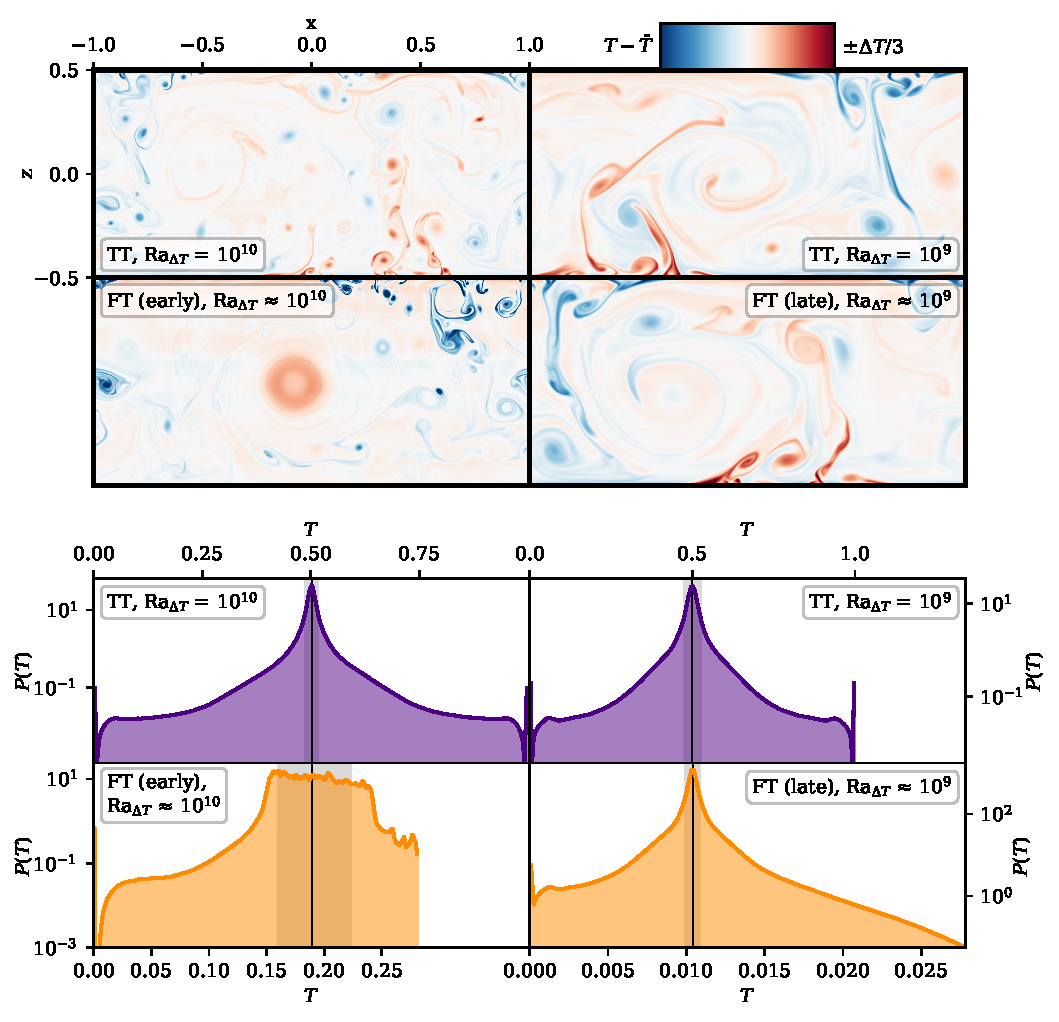
\includegraphics[width=\textwidth]{./figs/rbc_evolution_dynamics.pdf}
\caption{ 
	(Upper four panels) Snapshots of the temperature anomaly in two TT simulations (top row) and in an FT simulation at early and late times (bottom row).
	(Left two panels) Dynamics in a TT case at Ra$_{\Delta T} = 10^{10}$ and early in an FT simulation when Ra$_{\Delta T} \approx 10^{10}$.
	To first order, both cases have similar flow structures: a large convective cell and plumes which break apart into small turbulent eddies.
	However, in the FT case, the temperature anomaly of the cold plume is much larger than the hot plume, which does not appear on this color scale.
	(Right two panels) Dynamics in a TT case at Ra$_{\Delta T} = 10^9$ and in the relaxed state of the previously pictured FT simulation with Ra$_{\Delta T} \approx 10^9$.
	The relaxed FT simulation is visually indistinguishable from its comparable TT simulation.
\\	
	(Bottom four panels) Probability distribution functions (PDFs) of the full temperature field in each of the four dynamical panels pictured above.
	PDFs sample the dynamics in each simulation once every simulation freefall time unit over the course of 500 freefall time units.
	The black vertical line shows the median value, and the grey outline shows the 68\% confidence interval, or where the cumulative distribution function (CDF)'s value ranges from 0.16 to 0.84.
	(Top row) In both TT simulations, the temperature field has a mean value at $T = 0.5$ and a symmetric distribution around that peak with maxima at the fixed values of the boundaries. 
	(Bottom left) At early times in the FT simulation, the modal value of the PDF constantly moves left (towards the cold fixed-temperature boundary).
	(Bottom right) At late times, the temperature PDF from the cold fixed-temperature value (on the left) to the mode is indistinguishable from the TT PDF, but from the mode to the fixed-flux boundary there is a large tail characterized by low-probability, hot elements.
	\label{fig:rbc_evolution_dynamics} }
\end{figure}

In Fig.~\ref{fig:rbc_evolution_dynamics}, we compare the time evolution of the temperature field of an FT simulation with Ra$_{\partial_z T}$ = 4.83$\,\times 10^{10}$ to two TT simulations (with Ra$_{\Delta T} = 10^{10}$ and Ra$_{\Delta T} = 10^9$, respectively).
As shown in the top four panels, we see the expected convective roll solution in both TT simulations (top row) and at early and late times in the FT simulation (bottom row).
Interestingly, we find highly asymmetrical dynamics at early times in the FT simulation (bottom left), in which the temperature anomaly in the cold plume is much greater than in the warm plume.
This excess cold material slowly fills the domain and mixes, reducing the temperature difference between the top and bottom plates from $\Delta T = -1$ to $\Delta T = -\text{Nu}^{-1}$ in the relaxed state.
In this relaxed state, the supply of warm fluid from the bottom plume and cold fluid from the top plume come into balance, and the FT dynamics (bottom right) are indistinguishable from TT dynamics (top right).

In the bottom four panels, we examine these temperature fields statistically by displaying their probability distribution functions (PDFs).
To create these PDFs, we sample the full simulation temperature field once every freefall time unit\footnote{\ea{For TT simulations, a freefall time unit is one simulation time unit. For FT simulations, a freefall time unit is $\sqrt{\text{Nu}}$ simulation time units.}} over the span of 500 time units.
We interpolate the (unevenly spaced) vertical Chebyshev grid points onto an evenly spaced grid before histogramming the flow values into 200 bins and creating the PDFs.

We find that this statistical analysis of the simulations tells the same story as the dynamical images shown above.
The temperature field in both of the TT simulations (top row) is dominated by the modal temperature of 0.5 in the bulk; a smaller fraction of the domain is filled with equal portions of hotter/colder material (mostly contained in the plumes), and the temperature field is rigidly bounded by the fixed-temperature boundary values.
The story is more complex for the FT simulation.
At early times (lower left), the FT simulation is characterized by two features: an extreme tail (to the left) that characterizes the cold plume at the upper boundary, and a migrating modal temperature that shifts from the right (hotter) to the left (cooler) as cold material mixes in the interior.
At late times (lower right), the FT simulation's PDF is indistinguishable from the TT PDF between the cold (left), fixed-temperature boundary and the modal value.
From the modal value towards warmer temperatures, we find that the fixed-flux (lower boundary) is capable of producing more extreme temperature events and results in a more extended PDF tail.
This long tail is explored further in section \ref{sec:asymmetries}.

In the left panels of Fig.~\ref{fig:rbc_scalar_comparisons}, we examine the time evolution of scalar quantities from the FT simulation shown in Fig.~\ref{fig:rbc_evolution_dynamics} (orange lines) and compare it to the TT simulation with Ra$_{\Delta T} = 10^9$ (purples lines).
Simulation time is shown in nondimensional freefall units on the x-axis; the latest time displayed for each simulation, $t_{\text{final}}$, is subtracted for direct comparison of the relaxed states.
Traces of Ra$_{\Delta T}$ and Ra$_{\partial_z T}$ are shown in the top-left panel.
In the FT simulation, Ra$_{\Delta T}$ relaxes to its final value over thousands of simulation time units, and this final value is the input value of the equivalent TT case.
In comparison, Ra$_{\partial_z T}$ for the TT case instantaneously reaches its final value, which is the input value for the FT simulation.
This discrepancy in evolution timescales, where TT simulations evolve quickly and FT simulations evolve slowly, is also seen in the equilibration of Nu (middle panel) and Pe (bottom panel).

The right panels of Fig.~\ref{fig:rbc_scalar_comparisons} show that the relaxation of Ra$_{\Delta T}$ in FT simulations is akin to a sweep through Ra$_{\Delta T}$ parameter space.
The orange (Ra$_{\partial_z T} = 4.83 \times 10^{10}$, as on the left) and yellow (Ra$_{\partial_z T} = 2.61 \times 10^{9}$) lines show the evolution of FT simulations, and the arrows give the sense of time in the simulations.
For comparison, we plot results from TT simulations (purple circles) and the reported results of ref.~\cite{zhu&all2018} (black crosses).
The purple circles filled with orange and yellow circles are comparison TT simulations for the relaxed states of the FT simulations.
The top-right panel is a scaling plot for Nu vs.~Ra$_{\Delta T}$ compensated by the best fit reported in ref.~\cite{johnston&doering2009}.
The bottom-right panel is a scaling plot of Pe vs~Ra$_{\Delta T}$ compensated by the expected scaling \cite{ahlers&all2009}.
We find that FT simulations carry marginally more flux (higher Nu) and are more turbulent (higher Pe) than comparable TT simulations as they relax through this parameter space.
\ea{(TODO)}
%TODO: report scaling laws.
These heightened values of Nu and Pe suggest that the dynamics do not immediately ``forget'' the higher-Ra$_{\Delta T}$ state that they recently timestepped through on their way to achieving thermal relaxation.

Achieving thermal relaxation in pure FT simulations is computationally costly for two reasons: (1) the turbulent dynamics at the large initial Ra$_{\Delta T}$ require more spectral modes to resolve than the equilibrated state (compare the left and right dynamics in Fig.~\ref{fig:rbc_evolution_dynamics}), and (2) thousands of freefall times must pass during relaxation (see Fig.~\ref{fig:rbc_scalar_comparisons}).
For example, for the cases displayed in the left panels of Fig.~\ref{fig:rbc_scalar_comparisons} with a modest Ra$_{\Delta T} = 10^9$, the shown evolution of $10^4$ time units of the FT simulation cost $\sim 4.5 \times 10^5$ cpu-hours, while the TT equivalent case cost only $5.6 \times 10^4$ cpu-hours -- nearly an order of magnitude difference.
FT simulation dynamics evolve slowly during thermal relaxation, and these images, PDFs, and traces demonstrate the importance of waiting for thermal relaxation to be achieved when conducting an FT simulation.

\begin{figure}[t!]
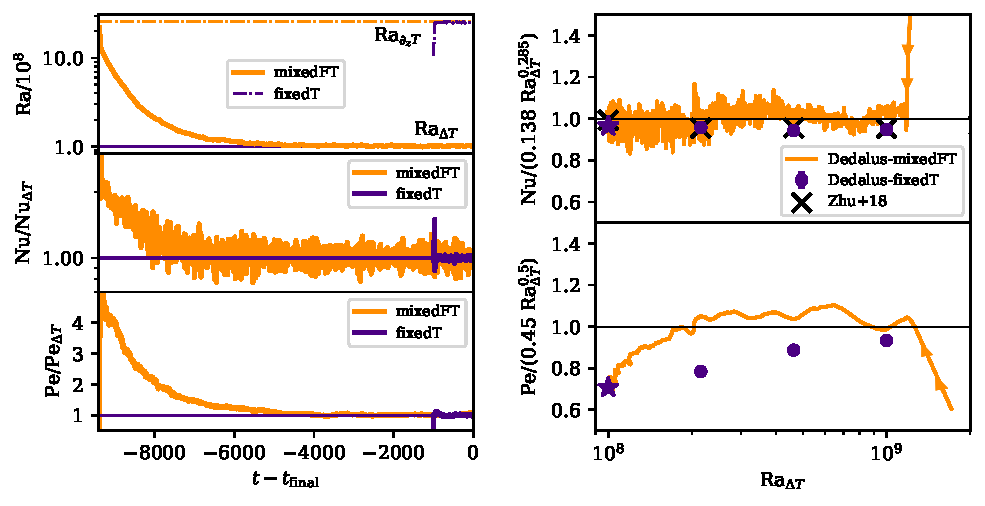
\includegraphics[width=\textwidth]{./figs/rbc_scalar_comparisons.pdf}
\caption{ 
	(Left three panels) Time traces of scalar quantities in an FT (orange) and TT (purple) simulation are shown.
	All traces have been averaged over a rolling window of 100 freefall time units to increase the clarity of the evolutionary trend.
	We display evolutionary traces of Ra (top, normalized by the input Ra$_{\Delta T}$ = $10^9$ value of the TT simulation) as well as Nu (middle) and Pe (bottom), both of which are normalized by their mean values measured over the last 500 freefall times of the TT simulation (reported in appendix \ref{app:table}).
	(Right two panels) Compensated scaling plots of Nu (upper) and Pe (lower) vs. Ra$_{\Delta T}$.
	Nu vs.~Ra is compensated by $(0.138 \text{Ra}_{\Delta T}^{0.285})$, the best-fit reported by ref.~\cite{johnston&doering2009}.
	Pe vs.~Ra is compensated by a Ra$_{\Delta T}^{1/2}$ law, the anticipated scaling of Pe \cite{ahlers&all2009}.
	The orange trace is the time evolution of the FT case from the left panels with the arrows showing the sense of time.
	The yellow trace shows the evolution of an FT case with Ra$_{\Delta T} = 10^8$.
	Purple circles are the measured values of Nu and Pe in our TT simulations (reported in appendix \ref{app:table}); error bars show the standard deviation of the sample mean and are smaller than the marker in all cases.
	The purple circles filled in with yellow and orange are the TT comparisons for the evolved states of the two FT cases.
	Black crosses show comparison TT simulations as reported by ref.~\cite{zhu&all2018}.
\label{fig:rbc_scalar_comparisons} }
\end{figure}



\subsection{TT-to-FT \& Nu-based ICs: rapidly equilibrated FT simulations}
\label{sec:tt-to-ft}

\begin{figure}
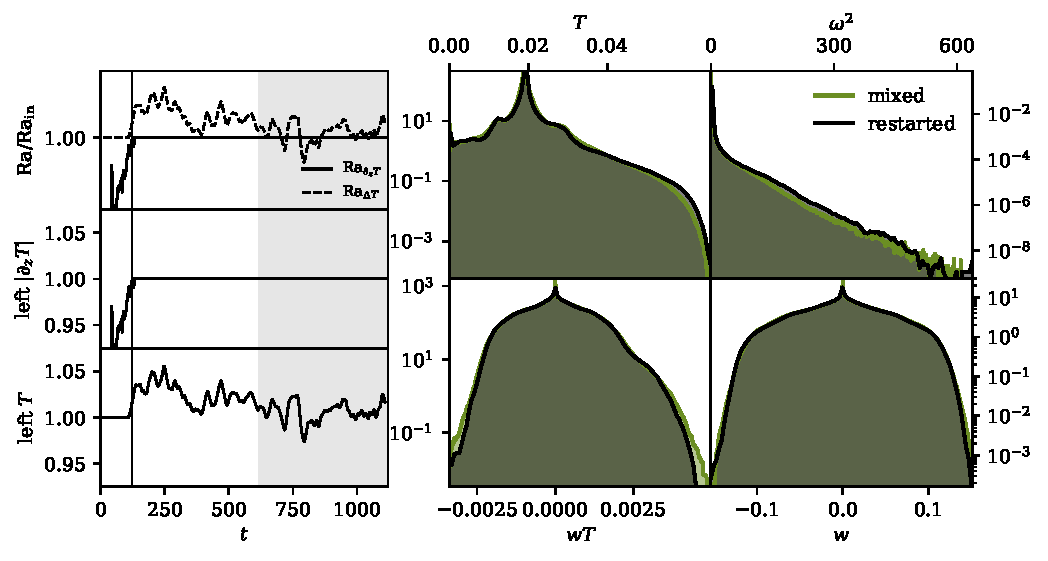
\includegraphics[width=\textwidth]{./figs/rbc_restart_description.pdf}
\caption{ 
	(Left three panels) Time traces of scalar quantities, which have been averaged over a rolling time window of 25 simulation time units, are shown for a simulation with Ra$_{\Delta T} = 10^9$ which starts with TT boundary conditions and then is switched to FT boundary conditions.
	The time of the change of boundary conditions is denoted by the vertical black line.
	(Top panel) The evolution of Ra is shown; Ra$_{\partial_z T}/(4.83\times 10^{10})$ is shown as a dashed-dot line, while Ra$_{\Delta T}/10^9$ is shown as a solid line.
	The mean value of temperature gradient (middle panel) and temperature (bottom panel) at the bottom boundary are also shown.
	In the TT initial state, the temperature is held constant at a value of 1 and the temperature derivative fluctuates around a value of $\text{Nu}$.
	In the FT final state, the temperature derivative is held constant at a value of -1 and the temperature value fluctuates around a value of $\text{Nu}^{-1}$.
	(right four panels) PDFs are shown which compare the dynamics during the grey time window in the left panels (black PDFs, TT-to-FT) to dynamics from a comparable time window in the FT case from Fig.~\ref{fig:rbc_scalar_comparisons}.
	We display the temperature field (upper left), enstrophy (upper right), nonlinear convective enthalpy flux (bottom left), and vertical velocity (bottom right).
\label{fig:rbc_restart_description} }
\vspace{-0.25cm}
\end{figure}

\ea{\paragraph{TT-to-FT} Figs.~\ref{fig:rbc_evolution_dynamics} \& \ref{fig:rbc_scalar_comparisons} demonstrate that the statistically-stationary states of FT and TT simulations are similar in a qualitative sense and in their volume-averaged flow statistics.}
It should therefore be possible to use results from a TT simulation to quickly reach the relaxed state of a comparable FT simulation, saving up to an order of magnitude in computational cost.
We show \ea{the results of using our TT-to-FT initial conditions procedure} in practice in Fig.~\ref{fig:rbc_restart_description}.
In the left three panels, we display the temporal behavior of (top) Ra, (middle) the flux at the bottom boundary, and (bottom) the temperature difference between the top and bottom boundaries.
We take the full evolution of the Ra$_{\Delta T} = 10^9$ TT simulation shown in Fig.~\ref{fig:rbc_scalar_comparisons}, then change its boundary conditions to FT at Ra$_{\partial_z T} = 4.83\times 10^{10}$.
The change from TT to FT boundaries occurs at the time denoted by the thin vertical line.
Unlike in the FT case displayed in Fig.~\ref{fig:rbc_scalar_comparisons}, there is no thermal rundown in the FT state, due to the rapid relaxation achieved during the TT portion of the simulation.

In the right four panels of Fig.~\ref{fig:rbc_restart_description}, we compare PDFs of flow fields in this TT-to-FT simulation and the comparable FT simulation which we timestepped through thermal relaxation.
Shown are PDFs of the temperature field (upper left), enstrophy (upper right), convective flux (lower left), and vertical velocity (lower right).
In Table~\ref{table:pdf_values}, we display the first four moments of each of these distributions,
\begin{equation}
\begin{split}
&\mu(A) \equiv \sum_{i} A_i\,P(A_i)\,\Delta A,\qquad\qquad\qquad\qquad\qquad\qquad\,\,
\sigma(A) \equiv \sqrt{\sum_{i}[A_i-\mu(A)]^2 P(A_i) \Delta A},\\
&\text{Skewness}(A) \equiv \frac{1}{\sigma(A)^3}\sum_i [A_i-\mu(A)]^3 P(A_i) \Delta A,\qquad
\text{Kurtosis}(A) \equiv \frac{1}{\sigma(A)^4}\sum_i [A_i-\mu(A)]^4 P(A_i) \Delta A,
\end{split}
\label{eqn:pdf_moments}
\end{equation}
where $A$ is a flow quantity, $P(A)$ is the PDF of $A$, $\mu$ is the mean, $\sigma$ is the standard deviation, $\Delta A$ is the spacing between the discrete PDF bins, and $i$ is the index of the bin.
\ea{We specifically report the Excess Kurtosis = Kurtosis $- 3$, to show how the Kurtosis of our PDFs differs from the Kurtosis of Normal Distributions.
The PDFs of all FT simulations agree well regardless of initial conditions, suggesting that all initial conditions do achieve a similar statistically stationary state.

\paragraph{Statistical Comparison of BCs and ICs}
From the moments of these PDFs, we conclude that the primary difference between FT and TT simulations is in the temperature field, and that the vertical velocities and nonlinear transport is the same regardless of boundary conditions.
The temperature PDF of the TT simulation unsurprisingly has a mean of 0.5, a Skewness close to zero (no asymmetry between upflows and downflows), and an appreciable Excess Kurtosis (the tails, which primarily sample the plumes, are more important than they are in a Normal Distribution).
The FT temperature PDF, on the other hand, has a small but noticeable skewness (suggesting asymmetries between the F and T plates), and more excess Kurtosis.
Furthermore, the mean temperature is slightly larger in the FT case.
Outside of the temperature field, we find that the vertical velocity, $w$, and the vertical heat transport, $wT$, are well-described by normal distributions  aside from the area near their peak of zero (which is dominated by the boundary layers).
}

\begin{table}[b!]
\vspace{-0.5cm}
\caption{ 
	The first four moments, as defined in Eqn.~\ref{eqn:pdf_moments}, of each of the PDFs shown in Fig.~\ref{fig:rbc_restart_description} are displayed below.
	\ea{Note that the coefficient resolution of the evolved FT simulation and the TT-to-FT simulation are the same (nz, nx) = (1024, 2048).}
}
\vspace{-0.25cm}
\setlength{\tabcolsep}{12pt}
\label{table:pdf_values}
\begin{center}
\begin{tabular}{c c c c c c c}
\hline																	
Quantity 				&	BCs	& ICs	    &	$\mu$					&	$\sigma$				&	Skewness	&	Excess Kurtosis \\
\hline
$T/\Delta T$			&	TT	& Classic	&	$5.00 \times 10^{-1}$	&	$7.11 \times 10^{-2}$	&	$-1.53 \times 10^{-2}$	&	$1.71 \times 10^{1}$ \\
						&	FT	& Classic	&	$5.07 \times 10^{-1}$	&	$7.37 \times 10^{-2}$	&	$7.31 \times 10^{-1}$	&	$2.40 \times 10^{1}$ \\
						&	FT	& TT-to-FT	&	$5.08 \times 10^{-1}$	&	$7.34 \times 10^{-2}$	&	$7.18 \times 10^{-1}$	&	$2.40 \times 10^{1}$ \\
						&	FT	& Nu-based	&	$5.06 \times 10^{-1}$	&	$7.36 \times 10^{-2}$	&	$7.63 \times 10^{-1}$	&	$2.40 \times 10^{1}$ \\
\hline                                                                                                                      
$\omega^2/\Delta T$		&	TT	& Classic	&	$3.99 \times 10^{2}$	&	$4.73 \times 10^{2}$	&	$5.87 \times 10^{1}$	&	$6.68 \times 10^{3}$ \\
						&	FT	& Classic	&	$9.30 \times 10^{2}$	&	$4.79 \times 10^{2}$	&	$8.13 \times 10^{1}$	&	$1.76 \times 10^{4}$ \\
						&	FT	& TT-to-FT	&	$6.37 \times 10^{2}$	&	$5.02 \times 10^{2}$	&	$6.56 \times 10^{1}$	&	$8.69 \times 10^{3}$ \\
						&	FT	& Nu-based	&	$6.94 \times 10^{2}$	&	$4.84 \times 10^{2}$	&	$7.27 \times 10^{1}$	&	$1.20 \times 10^{4}$ \\
\hline                                                                                                                      
$wT/(\Delta T)^{3/2}$	&	TT	& Classic	&	$1.46 \times 10^{-3}$	&	$1.63 \times 10^{-1}$	&	$5.14 \times 10^{-2}$	&	$5.85  \times 10^{-2}$ \\
						&	FT	& Classic	&	$1.53 \times 10^{-3}$	&	$1.69 \times 10^{-1}$	&	$3.28 \times 10^{-2}$	&	$-8.19 \times 10^{-2}$ \\
						&	FT	& TT-to-FT	&	$1.51 \times 10^{-3}$	&	$1.67 \times 10^{-1}$	&	$3.63 \times 10^{-2}$	&	$1.29  \times 10^{-1}$ \\
						&	FT	& Nu-based	&	$1.50 \times 10^{-3}$	&	$1.70 \times 10^{-1}$	&	$4.37 \times 10^{-2}$	&	$1.95  \times 10^{-1}$ \\
\hline                                                                                                                    
$w/(\Delta T)^{1/2}$ 	&	TT	& Classic	&	$-3.11 \times 10^{-5}$	&	$3.25 \times 10^{-1}$	&	$1.64 \times 10^{-2}$	&	$-1.16 \times 10^{-2}$ \\
						&	FT	& Classic	&	$-3.80 \times 10^{-5}$	&	$3.33 \times 10^{-1}$	&	$1.75 \times 10^{-3}$	&	$-1.48 \times 10^{-1}$ \\
						&	FT	& TT-to-FT	&	$2.66  \times 10^{-5}$	&	$3.29 \times 10^{-1}$	&	$-1.21 \times 10^{-3}$	&	$7.89  \times 10^{-2}$ \\
						&	FT	& Nu-based	&	$2.41  \times 10^{-5}$	&	$3.35 \times 10^{-1}$	&	$1.08 \times 10^{-2}$	&	$1.37  \times 10^{-1}$ \\
\hline																	
\end{tabular}
\end{center}
\end{table}


\ea{
\paragraph{Nu-based ICs}
The time evolution of Nu-based ICs is similar to the time evolution of TT simulations with classical ICs, with a few caveats.
The interior temperature gradient ($\grad_{\text{interior}}$ in Eqn.~\ref{eqn:nu_based_gradT}) is slightly positive at high Ra, which means that the interior is marginally thermally stable while the boundary layers are thermally unstable.
During the convective transient, plumes from the boundaries eat away at this interior stratification over a few tens of freefall timescales, after which time the interior is well mixed and a classical roll solution is achieved.
This behavior is quite different from classical ICs in TT simulations, in which the full domain is initially unstable and a roll solution is obtained immediately after the onset of nonlinear convection.
Regardless, the time required for the temperature field to reach statistical equilibrium is a few tens of freefall times rather than a few thousands of freefall times for classical ICs.
Per table \ref{table:pdf_values}, the evolved state of FT simulations with Nu-based ICs and classical ICs are very similar.
}


\subsection{\ea{Discussion of 2D results}} We note briefly that \ea{Nu-based ICs and} this TT-to-FT mechanism \ea{are} only \ea{two} of many ways of accelerating the thermal relaxation of an FT simulation.
We discuss other mechanisms, and explore one in detail, in our previous work \cite{anders&all2018}.
We note however that the TT-to-FT setup described here is likely the least complicated mechanism for achieving rapid relaxation in a simplified RBC setup that we are aware of.
The successful degree with which this mechanism reproduces the evolved dynamics suggests that thermal relaxation occurs in two parts:
\begin{enumerate}
\item Changes to the simulation energy reservoir, and
\item Restratification of the experiment.
\end{enumerate}
The thermal energy reservoir of TT simulations does not change between the initial and final state.
The rapid relaxation of TT simulations therefore suggests that experimental restratification occurs rapidly in RBC. 
The long rundown of FT experiments on display in Fig.~\ref{fig:rbc_scalar_comparisons} is entirely due to the energy reservoir (the mean temperature) drifting over time.
Put differently, the classic RBC setup for $T_0(z)$ is a bad choice of initial conditions for FT boundaries, and TT-to-FT simulations use TT dynamics to choose a more ideal set of initial conditions.
\ea{In practice, in this work, we find that the thermal relaxation of FT simulations with classical ICs takes $\sim 2.5\sqrt{\text{Ra}_{\partial_z T} \text{Pr}}\,\text{Nu}^{-1}$ simulation freefall time units.}

\ea{
As a final note, we find that measures of the velocity field (e.g., the kinetic energy and Pe) take a few hundred freefall timescales to relax to their final value in TT and FT (Nu-based IC) simulations in 2D at high values of Ra$\,\gtrsim 10^{8.67}$ .
This velocity field relaxation happens despite instant \emph{thermal} equilibration of the temperature field for these simulations.
We find that the kinetic energy increases by less than a factor of two from its initial post-transient value to its final value in the equilibrated state.
}

\begin{figure}[p!]
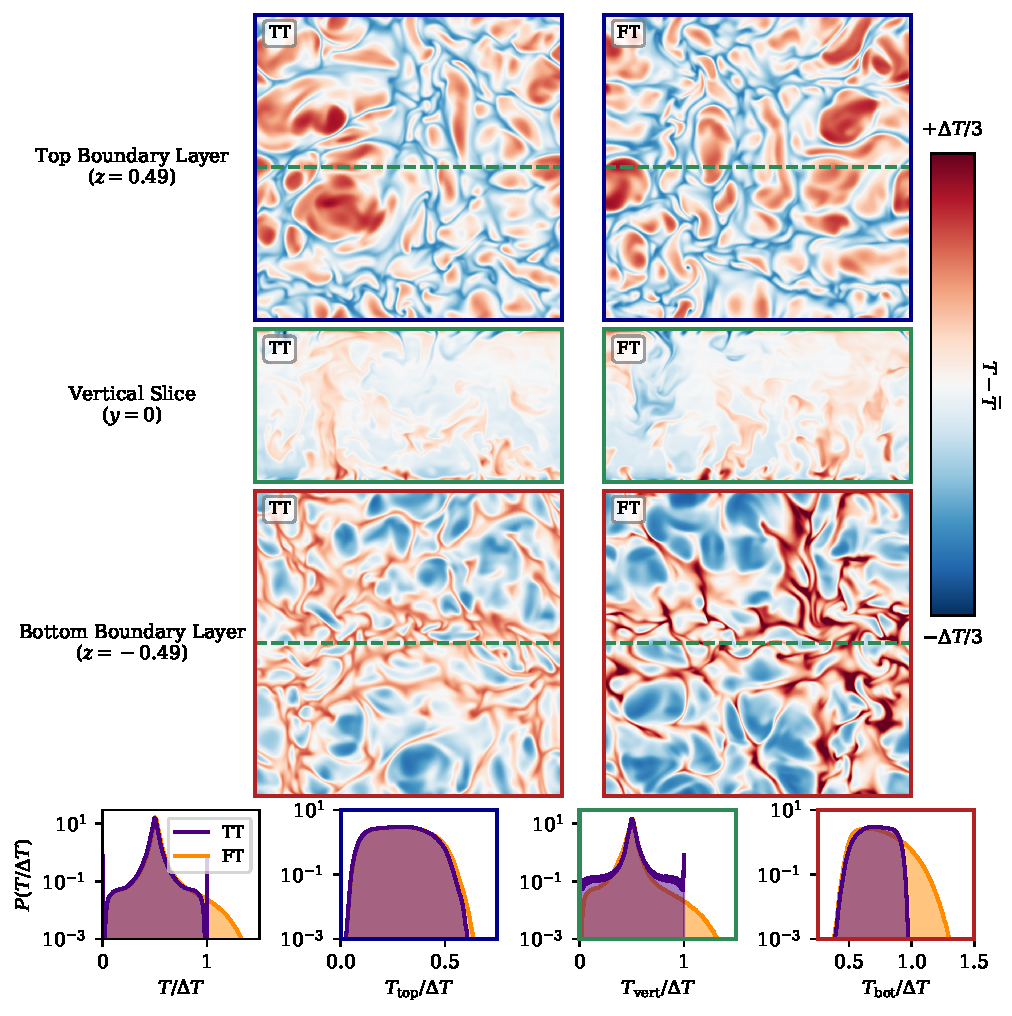
\includegraphics[width=\textwidth]{./figs/rbc_3D_panels.pdf}
\caption{ 
	(top six panels) Snapshots of the temperature anomaly are shown for select slices through 3D domains.
	The left column shows data from TT simulations with Ra$_{\Delta T} = 10^{8}$, the right column shows data for FT simulations with Ra$_{\partial_z T} = 3.1 \times 10^{9}$.
	The top and bottom rows respectively show horizontal slices 1\% of the domain depth away from the top and bottom boundaries, while the middle row shows a vertical slice at $y = 0$.
	Visually, TT and FT dynamics are indistinguishable aside from the warm upflows near the bottom boundary.
	(Bottom four panels) PDFs of the temperature field are shown.
	From left to right, these PDFs are shown for the full 3D domain, the upper boundary layer slice, the vertical slice, and the bottom boundary layer slice.
	The extreme temperature events which stand out visually near the bottom boundary layer can be clearly seen in all PDFs except for the one near the upper boundary.
	\label{fig:rbc_3D_panels} }
\end{figure}

\ea{
\subsection{3D verification of 2D results}
We note briefly that our results from 2D hold in 3D: classical ICs exhibit a prohibitively long thermal rundown, but equilibrated FT and TT simulations are analogous in a volume-averaged sense.
In Fig.~\ref{fig:rbc_3D_panels}, we show dynamical slices from a 3D TT and TT-to-FT simulation.
As in 2D, we find that the two simulations are nearly identical aside from their temperature fields, and so have focused on the temperature fields in this figure.
Near the top boundary and in the interior, the TT and FT dynamics are quite similar.
However, near the bottom boundary, the warm upflows in FT simulations are hotter relative to their counterparts in TT simulations.
At the bottom of the figure, we compare PDFs of the full temperature field to PDFs of the temperature field in each of the shown slices (near the top boundary layer, a vertical slice of the interior, and near the bottom boundary layer).
The PDF of the full volume of these simulations is indistinguishable between the two cases except near the hot bottom boundary.
Indeed, we find that the two cases have indistinguishable PDFs in a horizontal slice near the top boundary, and that temperature events which range from the fixed boundary temperature ($T = 0$) to the temperature achieved in the interior $T = 0.5\Delta T$) are all equally probable.
The story is the same for the TT case near the bottom boundary, but the FT case instead exhibits a slightly larger number of neutral events ($T = 0.5\Delta T$) in addition to extreme temperature events ($T \geq \Delta T$).
Unsurprisingly, we find that the PDF of the temperature field of a vertical slice through the domain at $y = 0$ is similar, but not identical, to the PDFs of the temperature field of the full volume, suggesting that this one slice does not capture the full range of possible dynamics which occur in the domain over our sampling window.
}

\FloatBarrier



\section{Results: Evolved dynamics and asymmetries in FT simulations}
\label{sec:results_dynamics}

\subsection{Evolved Structure}
\begin{figure}
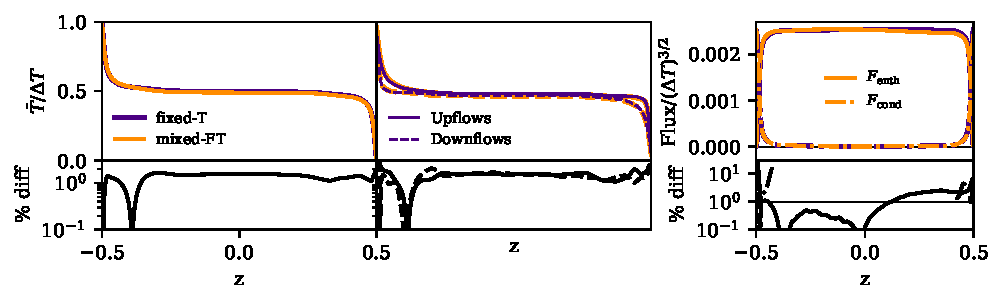
\includegraphics[width=\textwidth]{./figs/rbc_1D_profiles.pdf}
\caption{ 
	(Left three panels) We compare time- and horizontally-averaged profiles from an FT (orange) and TT (purple) simulation at Ra$_{\Delta T} = 10^{9}$.
	Shown are the (top) temperature, (middle) temperature in upflows (solid) and downflows (dashed), and (bottom) enthalpy (solid) and conductive (dashed) fluxes.
	The boundary layer regions are separated from the bulk by thin vertical lines and are examined in more detail in the right six panels.
	(Right six panels) The three panels on the left examine the bottom boundary layers and the right panels examines the top boundary layers.
	The insets show the \% difference between the FT and TT solutions.
	There are slight (a few \%) differences between the two cases near the bottom boundary, but otherwise the two cases are nearly the same to within $\sim 1$\%.
\label{fig:rbc_1D_profiles} }
\vspace{0.5cm}
\end{figure}

In Fig.~\ref{fig:rbc_1D_profiles}, we compare the time- and horizontally-averaged profiles of the temperature and fluxes in the evolved FT and TT cases presented in Fig.~\ref{fig:rbc_scalar_comparisons}.
Time averages are taken over 500 nondimensional freefall time units for the TT case and over 2000 nondimensional freefall time units for the FT case, sampled once every 0.1 time units (the difference in averaging window is explained in Sec.~\ref{sec:timescales}).
In the three left panels, we display profiles of (top) the mean temperature, (middle) the mean temperature in upflows (solid) and downflows (dashed), and (bottom) the convective enthalpy flux ($F_{\text{enth}} = wT$, solid) and the conductive flux ($F_{\text{cond}} = -\Peff^{-1}\grad T$, dashed).
Most of the interesting structure is in the boundary layers, located between the sides of the plots and the thin vertical black lines.
Zoomed in plots of the bottom and top boundary layers are respectively shown in the middle and right columns.
Inset panels show the percentage difference between the FT and TT solutions.
In the flux panels (bottom row), we do not plot the percentage difference in the conductive flux, as this quantity is undefined in the bulk of the interior where that flux is zero.
The conductive flux of the two cases agrees to within a few \% in the boundary layers, and the largest deviations away from zero in the interior are O(0.01) in the plotted units. 

We find good ($\sim 1\%$) agreement between the FT and TT temperature profiles and enthalpy fluxes throughout the full depth of the domain, with slightly larger differences near the bottom boundary where the boundary conditions differ.
When we split the temperature profile into upflows and downflows, we find that FT upflows/downflows are slightly warmer/cooler than their TT counterparts at the hot, bottom boundary.
These differences are interesting, and are explored further in section \ref{sec:asymmetries} and Fig.~\ref{fig:rbc_dynamics_asymmetries}, but vanish in the interior and do not likely affect the convective dynamics appreciably.



\subsection{Asymmetries induced by mixed boundaries}
\label{sec:asymmetries}

\begin{figure}
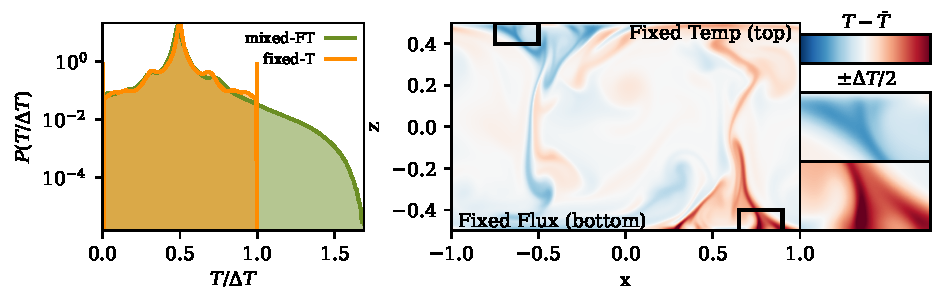
\includegraphics[width=\textwidth]{./figs/rbc_dynamics_asymmetries.pdf}
\caption{ 
	(Left panel) PDFs of temperature measurements of a TT-to-FT (orange) and TT (purple) case with Ra$_{\Delta T} = 10^{10}$ are displayed.
	The right tail of the distribution (near the hot fixed-flux boundary for the FT case) shows that fixed flux boundaries achieve more extreme temperature events than fixed temperature boundaries.
	(Middle panel) A snapshot of the temperature anomaly in the FT simulation.
	Zoomed in views of the regions outlined in black boxes are shown in the right two panels.
	Near the top (fixed temperature) boundary, the temperature anomaly at the root of the plume vanishes, but this does not happen near the bottom (fixed flux) boundary, allowing for more extreme instantaneous values.
\label{fig:rbc_dynamics_asymmetries} }
\end{figure}

We now study in more detail the asymmetries introduced into a solution by FT boundaries.
We run a TT and TT-to-FT simulation at Ra$_{\Delta T} = 10^{10}$ and Ra$_{\partial_z T} = 9.51 \times 10^{11}$, respectively.
In Fig.~\ref{fig:rbc_dynamics_asymmetries}, we examine the dynamical nature of the asymmetries which FT boundaries introduce into the simulation near the fixed-flux boundary.
In the left panel, we plot PDFs of the temperature fields in comparable TT and FT simulations.
These PDFs agree remarkably well near the mean and for cold temperatures (near the fixed temperature boundary), but diverge in the tail of the PDF for hot temperatures where $T/\Delta T \gtrsim 0.8$, where the boundary conditions differ.
Interestingly, there are no temperature fluctuations which exceed the specified boundary values in the convective domain for TT simulations.
However, the FT PDF has a much longer tail and the FT solution achieves fluid parcels which are hotter than the average bottom boundary value by more than 50\%.
In order to understand how this is possible, we examine a snapshot of the FT simulation's temperature anomaly in the middle panel.
We have outlined a portion of a cold plume near the upper (fixed-temperature) boundary and a portion of a hot plume near the lower (fixed-flux) boundary, and these regions are magnified in the rightmost panels.
The TT upper boundary suppresses temperature anomaly at the upper boundary and regulates the temperature minima which can be achieved.
The fixed-flux lower boundary does no such suppression and allows for extreme temperature values to be achieved in the plume-launching area, thus allowing for the asymmetry in the tails of the temperature PDF.

We note briefly that these asymmetries do not seem to affect mean or volume-averaged quantities in these simulations appreciably (see the agreement between FT and TT in Figs.~\ref{fig:rbc_scalar_comparisons}\&\ref{fig:rbc_1D_profiles}).
However, the fact that fixed-flux boundaries produce a wider temperature distribution with more extreme values may be important in some astrophysical studies.
We explore this further in the discussion in section \ref{sec:discussion}.





\section{Results: Rotating \RB Convection}
\label{sec:results_rotating}

We now extend our study to a more complicated experiment: 3D rotating RBC with an Ekman number of $10^{-6}$.
We study a TT case at Ra$_{\Delta T} = 2.75\times 10^9$, and an FT case at $\text{Ra}_{\partial_z T} = 2.1 \times 10^{10}$ (the supercriticality of the TT case is $\sim 3$).
\footnote{\ea{At these parameters, we would be in the cellular convection regime of \citet{stellmach&all2014}, but our dynamics are different due to our choice of stress free boundary conditions.
}}.
These simulations employ stress free boundary conditions which allow for the generation of mean flows such as large scale vortices (LSV) \ea{\citep{stellmach&all2014, rubio&all2014, guervilly&all2014, guervilly&hughes2017, favier&all2014, favier&all2019, couston&all2019}}.

In the left three panels of Fig.~\ref{fig:rotating_panels}, we compare the time evolution of the FT and TT cases.
The top left panel shows the evolution of Ra$_{\partial_z T}$ and Ra$_{\Delta T}$.
Even in the presence of strong rotation, the TT immediately equilibrates, but the FT case takes thousands of freefall times to achieve thermal relaxation.
In the middle panel, we show the evolution of Ro; the evolved flows in both simulations exhibit rotationally constrained dynamics with Ro $\,\approx 0.1$, but the flows in the FT simulation relax to this state from an initially unconstrained state (Ro $\,\approx 1$).
This implies that the thermal relaxation process can walk through the parameter space of flow balances (e.g., the balance between Inertial and Coriolis forces) in addition to the Ra$_{\Delta T}$ parameter space.
In the bottom panel, we display the evolution of Pe over time.
Strangely, the peak value of Pe occurs a few hundred freefall times after the convective transient.
After achieving this peak value, Pe monotonically decreases toward its relaxed state.

In the upper right panel of Fig.~\ref{fig:rotating_panels}, we plot Nu vs.~Ra for rotating simulations.
Select TT cases are plotted as cyan circles with purple outlines (where the cyan color denotes the value of Ek$\,=\,10^{-6}$ according to the color bar).
The evolution of the FT case in the left panels is shown as a thick orange line with a cyan interior and the black arrows show the direction of time.
The TT case that corresponds to the FT case is a purple star with a cyan interior.
We have additionally included some literature data from numerical simulations (circles) and experiments (diamonds) as reported in the appendix tables of ref.~\cite{cheng&all2015}.
These experiments were conducted in a cylindrical geometry at a different Pr, and are not meant to be one-to-one-comparable, but are meant to guide the eye to the nature of the parameter space of rotating convection.
The solid black line is the best-fit line for rotationally unconstrained simulations with Ra $\geq 10^{10}$ from ref.~\cite{cheng&all2015}.
As expected, the scaling of Nu vs.~Ra is steep in the rotationally constrained regime \cite{julien&all2012, plumley&julien2019}, which these simulations trace through.
As in Fig.~\ref{fig:rbc_scalar_comparisons}, the FT values of Nu are once again somewhat elevated above the comparable TT simulations.

In the bottom right three panels of Fig.~\ref{fig:rotating_panels}, we plot the vertically integrated vertical vorticity in the simulation at three different times.
In the left panel, a dominant LSV which is aligned with the global rotation dominates the simulation at early times.
Over thousands of freefall times, this LSV evolves into a long-lived vortex pair, displayed in the middle panel.
Finally, in the evolved state, this vortex pair solution begins to oscillate with domain-wide jets, such as those displayed in the right panel.
We find that the TT solution shows this oscillatory behavior between vortex pairs and jets immediately and throughout the full 5000 freefall timescales of evolution that we simulated.

We suspect that the strange behavior of Pe in the bottom left panel can be explained by the evolution of the dominant flow structures over time.
At early times, the initially large value of Ra$_{\Delta T}$ in the FT case drives the displayed dominant LSV.
This powerful driving injects energy into the LSV, causing Pe to grow.
As Ra$_{\Delta T}$ and convective driving decrease over time, the LSV saturates and then starts to wind down, leading to the ``bump'' in the Pe trace.

We once again find it important to briefly note the difference in computational cost between the FT and TT simulations conducted here.
The TT simulation shown in the left panels of Fig.~\ref{fig:rotating_panels} only cost $2.6 \times 10^4$ cpu-hours.
By comparison, the cost of the FT simulation shown in the same panels was \emph{two orders of magnitude larger}---$2.3 \times 10^6$ cpu-hours.
The TT simulation's coefficient resolution was $128^3$.
The FT simulation's initial resolution required to resolve the convective transient was $512\times384^2$ coefficients.
We reduced the resolution to $256\times384^2$ after 100 freefall times, and then later to $128\times384^2$ after $\sim3.3 \times 10^3$ freefall times.
At each of these times, we found that lowering the \emph{horizontal} coefficient resolution of the simulation did not reproduce the simulation solution with fidelity.
This suggests that small scale turbulent velocity structures---which are injected by the vigorous transient and perhaps associated with the LSV---are long lived throughout the thermal evolution of the simulation.

\begin{figure}
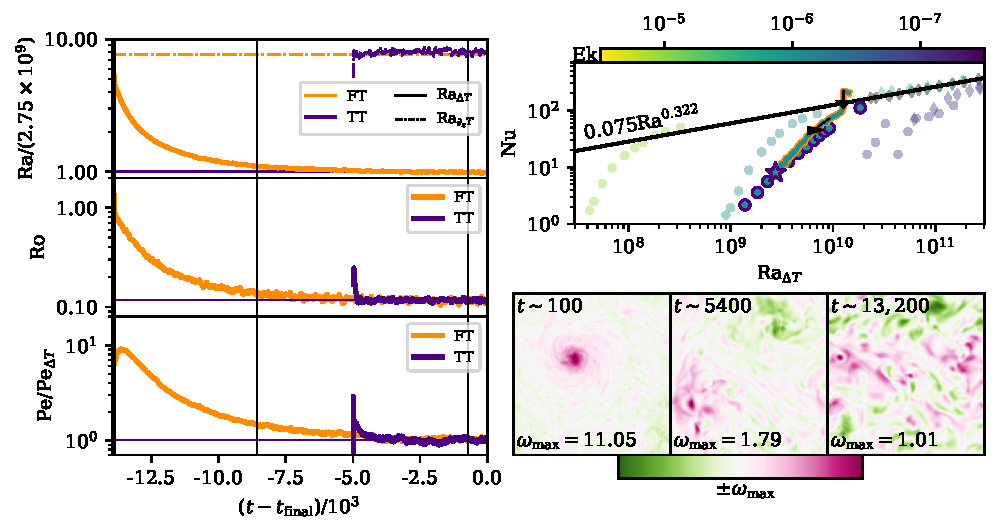
\includegraphics[width=\textwidth]{./figs/rotating_panels.pdf}
\caption{ 
	(Left three panels) Time traces of scalar quantities in an FT (orange) and TT (purple) simulation are shown.
	All traces have been averaged over a rolling window of 50 freefall time units to increase the clarity of the evolutionary trend.
	(Top panel) Ra, normalized by the input Ra$_{\Delta T}$ = 2.75$\,\times 10^9$ of the TT simulation.
	(Middle panel) Ro evolution of both simulation; the bulk flow of the FT simulation transitions from a marginally rotationally unconstrained state to a constrained state, while the TT simulation is always rotationally constrained.
	(Bottom panel) Pe evolution of the simulations is shown, normalized by the mean value measured over the last 500 freefall times of the TT simulation.
	(Upper right panel) Parameter space of Nu vs.~Ra$_{\Delta T}$ in rotating convection.
	Circular and diamond data points are respectively simulations and experimental data points from \cite{cheng&all2015}.
	The color of the data points signifies the Ekman number of the points, and black points are non rotating.
	Data from our Ek$\,=\,10^{-6}$ FT experiment are shown as a thick orange line with a cyan interior, where the black arrows give the direction of time.
	Some TT simulations are shown as purple circles with a cyan interior, and the TT case which corresponds to the relaxed state of the FT simulation is shown as a star.
	(Bottom right panels) Snapshots of the vertically integrated z-component of the vorticity from the FT simulation.
	At early times (left panel), a powerful large scale vortex with positive vorticity develops.
	This vortex slowly decays and becomes a vortex pair (middle panel), as seen in ref.~\cite{stellmach&all2014}.
	In the converged state, we see oscillatory behavior between this vortex pair behavior and jets (right panel).
	The TT case exhibits the oscillatory behavior between vortex pairs and jets throughout its whole evolution.
	The three vertical black lines in the left panels signify the times at which these snapshots are taken.
\label{fig:rotating_panels} }
\end{figure}




%%%%%%%%%%%%
%%%%%%%%%%%
% CONCLUSION
%%%%%%%%%%%
%%%%%%%%%%%%

\section{Conclusions \& Discussion}
\label{sec:discussion}
In short, we find that FT simulations experience a long thermal relaxation which is not experienced by TT simulations and, to first order, FT boundaries do not introduce important asymmetries into the solution.

In this paper, we have studied the time evolution of \RB convection (RBC) under two different formulations of the thermal boundary conditions: ``FT'' boundaries, where the flux is fixed at the bottom and temperature is fixed at the top, and ``TT'' boundaries, where temperature is fixed at the top and bottom.
Through studying this relaxation and the relaxed states of both simulations, we come to the following conclusions:
\begin{enumerate}
\item Thermal relaxation in RBC has two components: (a) changes in the energy reservoir and (b) changes in the stratification.
We find that the long relaxation of FT simulations is due to changes in the energy reservoir; this reservoir is roughly constant in TT simulations due to the lack of evolution of the average domain temperature.
The rapid evolution of our TT simulations suggests that RBC restratifies itself instantaneously.
\item Dynamical measurements taken during the thermal relaxation of an FT simulation may be misleading.
Dynamics during the relaxation are more turbulent than in the evolved state, and exhibit evolving flow balances in the equation of motion (as quantified by e.g., the Rossby number).
\item The thermal relaxation process of an FT simulation performs a sweep through Ra$_{\Delta T}$ parameter space.
We find that convective heat transport (the Nusselt number) and turbulent velocities (the P\'{e}clet number) are elevated above classical scaling laws along these parameter space sweeps.
\item Great computational expense achieving thermal relaxation in an FT simulation can be avoided by using the evolved state of a TT simulation as a ``better'' set of initial conditions for an FT simulation.
\item Despite minor asymmetries near the fixed-flux boundary, we find no meaningful difference between the mean state of FT and TT simulations.
\end{enumerate}
We now describe some lessons that should be applied from this work to astrophysical convection, and comment on some open areas of research.

Throughout this work, we have made the assumption that convection is only ``interesting'' in its final, fully equilibrated state.
In nature, convection is not always in an equilibrium state.
For example, in the late stages of the lifetimes of stars, some core burning regions have sufficiently short lifetimes that they likely do not come into thermal relaxation \citep{clarkson&all2018, andrassy&all2020}.
The use of FT boundaries or initial conditions that we have here considered to be ``bad'' choices may help in understanding these transient lifetime stages.
However, for most convective studies where the lifetime of the natural convective system is much larger than its Kelvin-Helmholtz timescale, it is essential to study relaxed convection, and our results point towards the importance of either choosing good initial conditions (TT or TT-to-FT simulations) or running simulations to thermal relaxation.

One question which our study of RBC is not able to address is: how long does it take for a complex convective system to restratify?
Our fully convective domains restratified instantaneously, but it is likely that mixed convective-and-stably-stratified domains \citep{brummell&all2002, kapyla&all2019, pratt&all2017, korre&all2019} should have regions that are not turbulently mixed by convection which could also have long relaxation timescales.
It would be extremely helpful for future studies to examine relaxational timescales in systems where the energy reservoir is fixed, but where convection does not effectively mix the whole domain.
Fortunately, clever techniques (e.g., as we explored in ref.~\cite{anders&all2018}) can likely be used to rapidly restratify atmospheres in such simulations.

RBC is fundamentally symmetrical, but many natural convective processes occur in density-stratified domains in which the symmetries of the problem are fundamentally broken.
In the present study, we observed that flux boundaries produce more extreme thermodynamic events than temperature boundaries.
In studies of overshooting convection, it is possible that plumes produced by a flux boundary layer could launch further into a stable layer than plumes produced by a temperature boundary.
Some authors have aimed to quantify the nature of overshooting plumes from a convective region into a stable region \cite{pratt&all2017, korre&all2019}, and it is unclear if different choices of boundary conditions could change the observed distribution of overshooting plumes observed there.

Some of the most complex astrophysical convection experiments aim to understand self-consistently evolving magnetic dynamos in rotating, spherical, magnetohydrodynamical domains \cite{brown&all2010, yadav&all2016, strugarek&all2017, strugarek&all2018}.
These dynamo simulations involve large numbers of timesteps through many freefall timescales in order to study the generation and evolution of magnetic fields and mean flows.
We found in our FT rotating simulation that the unrelaxed state generated a mean flow (a LSV, Fig.~\ref{fig:rotating_panels}) that was much more intense and large-scale than the eventual flows that developed in the relaxed state.
If we had terminated our FT rotating simulation too early, we would not have seen the eventual destruction of this LSV or the later oscillatory behavior between jets and vortex pairs.
Many dynamo simulations are performed in highly turbulent regimes at the cutting-edge of what is achievable using modern computational resources.
As a result, timestepping through thousands of freefall timescales is not possible in these simulations.
It is therefore crucial that dynamo simulations be set up in such a manner as to avoid large changes to the system's energy reservoir such as those that we observed and studied here.
Some authors who study astrophysical convection \citep{featherstone&hindman2016a, strugarek&all2018, bordwell&all2018, matilsky&all2019} employ FF boundary conditions, and our results here suggest that such a choice may be ideal in those complex simulations.

In conclusion, we note that our results here should provide astrophysical convection simulations with reason for optimism.
Some problems that we encounter (e.g., long thermal rundown in FT simulations) can be completely avoided through a careful understanding of the numerical system being solved.

\begin{acknowledgments}
We'd like to thank Daniel Lecoanet, who first pointed out to us the importance of examining Ra$_{\Delta T}$ in FT simulations. 
We'd also like to thank Jeff Oishi, who encouraged us to pursue the differences between early and late FT dynamics and who graciously saved the reader from reading ``mixedFT'' (instead of FT) and ``fixedT'' (instead of TT).
EHA acknowledges that this work was supported by NASA Headquarters under the NASA Earth and Space Science Fellowship Program -- Grant 80NSSC18K1199.
LK acknowledges support from the George Ellery Hale Post-Doctoral Fellowship.
This work was additionally supported by NASA LWS grant NNX16AC92G and by the National Science Foundation under grant No.~1616538. 
Computations were conducted with support by the NASA High End Computing (HEC) Program through the NASA  Advanced Supercomputing (NAS) Division at Ames Research Center on Pleiades with allocation GID s1647.
\end{acknowledgments}


\bibliography{biblio.bib}

\appendix
\section{Table of Simulations}
\label{app:table}
Input and output information for the simulations in this work are shown in Table~\ref{table:simulations}.
The codes used to run these simulations can be found online in the repository of supplemental materials \cite{anders&all2020a_supp}.



\begin{table}[ht]
\caption{
	Input and output values from the simulations in this work are shown; all simulations have a Prandtl number of 1.
	Input quantities are the boundary conditions (BCs), Rayleigh number (Ra), coefficient resolution (nx$\times$ny$\times$nz, or horizontal $\times$ vertical), and the total simulation run time in freefall units $t_{\text{simulation}}$ and in cpu-hours.
	Output quantities are the Nusselt (Nu), P\'{e}clet (Pe), and Rossby (Ro) numbers.
	Reported values of Nu, Re, and Ro are the sample mean over the last 500 freefall time units.
	Reported uncertainties are the standard deviation of the sample mean; when the uncertainty is not reported, it is smaller than the number of reported digits.
	The ``Nu comp'' values are comparison Nu values reported in ref.~\cite{zhu&all2018}.
	Resolutions marked by a $*$ show the initial, highest resolution utilized in the simulation.
	The 2D FT Ra = $4.83 \times 10^{10}$ simulation's resolution was changed to $1024\times2048$ about 500 freefall time units after transient.
	The rotating FT case's resolution was reduced to $384^2\times256$ about one hundred freefall time units after transient, and was further reduced to $384^2\times128$ about $3.3\times 10^3$ freefall times after transient.
}
\setlength{\tabcolsep}{8pt}
\label{table:simulations}
\begin{center}
\resizebox{\textwidth}{!}{
\begin{tabular}{c c c c c c c c c}
\hline																	
BCs	&	Ra	&	nx$\times$ny$\times$nz	& $t_{\text{simulation}}$	&	cpu-hours 	&	Nu	&	Nu comp	&	Pe  & Ro \\
\hline \hline \multicolumn{6}{c}{\vspace{-0.2cm}}\\
\multicolumn{7}{c}{\vspace{0.1cm}2D Runs ($\Gamma = 2$, no-slip)} \\
\hline
TT			&	$1.00 \times 10^8$		&	1024x512	&	1023		&	$5.57 \times 10^3$	&	$25.4 \pm 0.1$	&	26.1	&	$3.18 \times 10^3$ & --- \\
FT			&	$2.61 \times 10^9$		&	2048x1024	&	9410		&	$1.21 \times 10^5$	&	$25.3 \pm 0.2$	&	26.1	&	$3.31 \times 10^3$ & --- \\
TT-to-FT	&	$2.61 \times 10^9$		&	1024x512	&	1000		&	$1.88 \times 10^3$	&	$26.1 \pm 0.1$	&	26.1	&	$3.22 \times 10^3$ & --- \\
TT			&	$2.15 \times 10^8$		&	1024x512	&	1023		&	$5.73 \times 10^3$	&	$31.3 \pm 0.2$	&	31.2	&	$5.17 \times 10^3$ & --- \\
TT			&	$4.64 \times 10^8$		&	2048x1024	&	1024		&	$4.66 \times 10^4$	&	$38.4 \pm 0.3$	&	38.9	&	$8.60 \times 10^3$ & --- \\
TT			&	$1.00 \times 10^9$		&	2048x1024	&	1023		&	$5.58 \times 10^4$	&	$48.0 \pm 0.4$	&	48.3	&	$1.33 \times 10^4$ & --- \\
FT			&	$4.83 \times 10^{10}$	&	4096x2048*	&	16230		&	$5.36 \times 10^5$	&	$48.7 \pm 0.4$	&	48.3	&	$1.41 \times 10^4$ & --- \\
TT-to-FT	&	$4.83 \times 10^{10}$	&	2048x1024	&	1000		&	$1.11 \times 10^4$	&	$48.7 \pm 0.3$	&	48.3	&	$1.36 \times 10^4$ & --- \\
TT			&	$2.15 \times 10^9$		&	2048x1024	&	1029		&	$6.38 \times 10^4$	&	$60.4 \pm 0.5$	&	61.1	&	$1.99 \times 10^4$ & --- \\
TT			&	$4.64 \times 10^9$		&	3072x1536	&	1024		&	$3.29 \times 10^5$	&	$75.2 \pm 0.6$	&	76.3	&	$2.94 \times 10^4$ & --- \\
TT			&	$1.00 \times 10^{10}$	&	4096x2048	&	1039		&	$7.79 \times 10^5$	&	$95.3 \pm 0.7$	&	95.1	&	$4.30 \times 10^4$ & --- \\
TT-to-FT	&	$9.51 \times 10^{11}$	&	4096x2048	&	1000		&	$7.91 \times 10^4$	& 	$93.2 \pm 0.8$ 	&	95.1	&	$4.11 \times 10^4$ & --- \\
\hline																	
\multicolumn{7}{c}{\vspace{0.1cm}3D Rotating Runs (Ek = $10^{-6}$, $\Gamma = 0.481$, stress-free)} \\
\hline																	
TT	&	$1.38 \times 10^9$		&	64$^2\times$128 	&	2565		&	$2.98 \times 10^3$	&	$2.17$			&	---		&	$2.84 \times 10^2$  & $(3.38 \pm 0.17) \times 10^{-2}$ \\
TT	&	$1.83 \times 10^9$		&	64$^2\times$128 	&	2545		&	$3.54 \times 10^3$	&	$3.56$			&	---		&	$5.28 \times 10^2$  & $(5.67 \pm 0.33) \times 10^{-2}$ \\
TT	&	$2.29 \times 10^9$		&	128$^3$				&	2537		&	$1.08 \times 10^4$	&	$5.61$			&	---		&	$8.91 \times 10^2$  & $(8.56 \pm 0.44) \times 10^{-2}$ \\
TT	&	$2.75 \times 10^9$		&	128$^3$				&	5035		&	$2.6 \times 10^4$	&	$8.04 \pm 0.01$	&	---		&	$1.71 \times 10^3$  & $(1.17 \pm 0.06) \times 10^{-1}$ \\
FT	&	$2.1 \times 10^{10}$	&	384$^2\times$512*	&	13950		&	$2.3 \times 10^6$	&	$7.86 \pm 0.01$	&	---		&	$1.76 \times 10^3$  & $(1.14 \pm 0.06) \times 10^{-1}$ \\
TT	&	$3.67 \times 10^9$		&	128$^3$				&	2532		&	$1.55 \times 10^4$	&	$12.5$			&	---		&	$3.39 \times 10^3$  & $(1.74 \pm 0.08) \times 10^{-1}$ \\
TT	&	$4.58 \times 10^9$		&	128$^3$				&	2530		&	$1.69 \times 10^4$	&	$17.6$			&	---		&	$4.77 \times 10^3$  & $(2.35 \pm 0.08) \times 10^{-1}$ \\
TT	&	$5.50 \times 10^9$		&	192$^3$				&	2402		&	$7.35 \times 10^4$	&	$22.8$			&	---		&	$6.38 \times 10^3$  & $(2.96 \pm 0.11) \times 10^{-1}$ \\
TT	&	$6.42 \times 10^9$		&	192$^3$				&	2226		&	$7.35 \times 10^4$	&	$29.5$			&	---		&	$7.86 \times 10^3$  & $(3.65 \pm 0.16) \times 10^{-1}$ \\
TT	&	$7.33 \times 10^9$		&	256$^3$				&	1147		&	$1.47 \times 10^5$	&	$36.2$			&	---		&	$9.52 \times 10^3$  & $(4.33 \pm 0.17) \times 10^{-1}$ \\
TT	&	$8.25 \times 10^9$		&	256$^3$				&	1079		&	$1.47 \times 10^5$	&	$43.0$			&	---		&	$1.10 \times 10^4$  & $(5.01 \pm 0.20) \times 10^{-1}$ \\
TT	&	$9.17 \times 10^9$		&	256$^3$				&	1030		&	$1.47 \times 10^5$	&	$48.9$			&	---		&	$1.24 \times 10^4$  & $(5.63 \pm 0.26) \times 10^{-1}$ \\
TT	&	$1.834 \times 10^{10}$	&	256$^3$				&	971.9		&	$1.84 \times 10^5$	&	$111$			&	---		&	$2.21 \times 10^4$  & $1.18 \pm 0.09$ \\
\hline																	
\end{tabular}
}
\end{center}
\end{table}



\end{document}
